\documentclass{article}
\usepackage{graphicx}
\usepackage{fancyvrb}

\begin{document}
\tableofcontents
\section{Coding}
You can try your main loop without scheduling events by setting the \verb+schedulingFlag+ to false.
\section{The components of the system}
This model aims at reproducing the dynamics of an economic systems.

Describing the functioning of a dynamic system implies to know the components of the systems, how they work and how they interact with each other. 
Therefore it is a demanding task.

To ease the task, we report hereafter two visual representations. The first one aims at showing the \textbf{model components} and the second one describes the \textbf{sequence of events} in each time step.

The reader can overview these two visual representations by looking at figures \ref{fig:components} and \ref{fig:sequence}.

In the following subsections we will carefully describe these two representations because they will be used in combination throughout the whole document. 

\begin{figure}[htp]
\hskip-1cm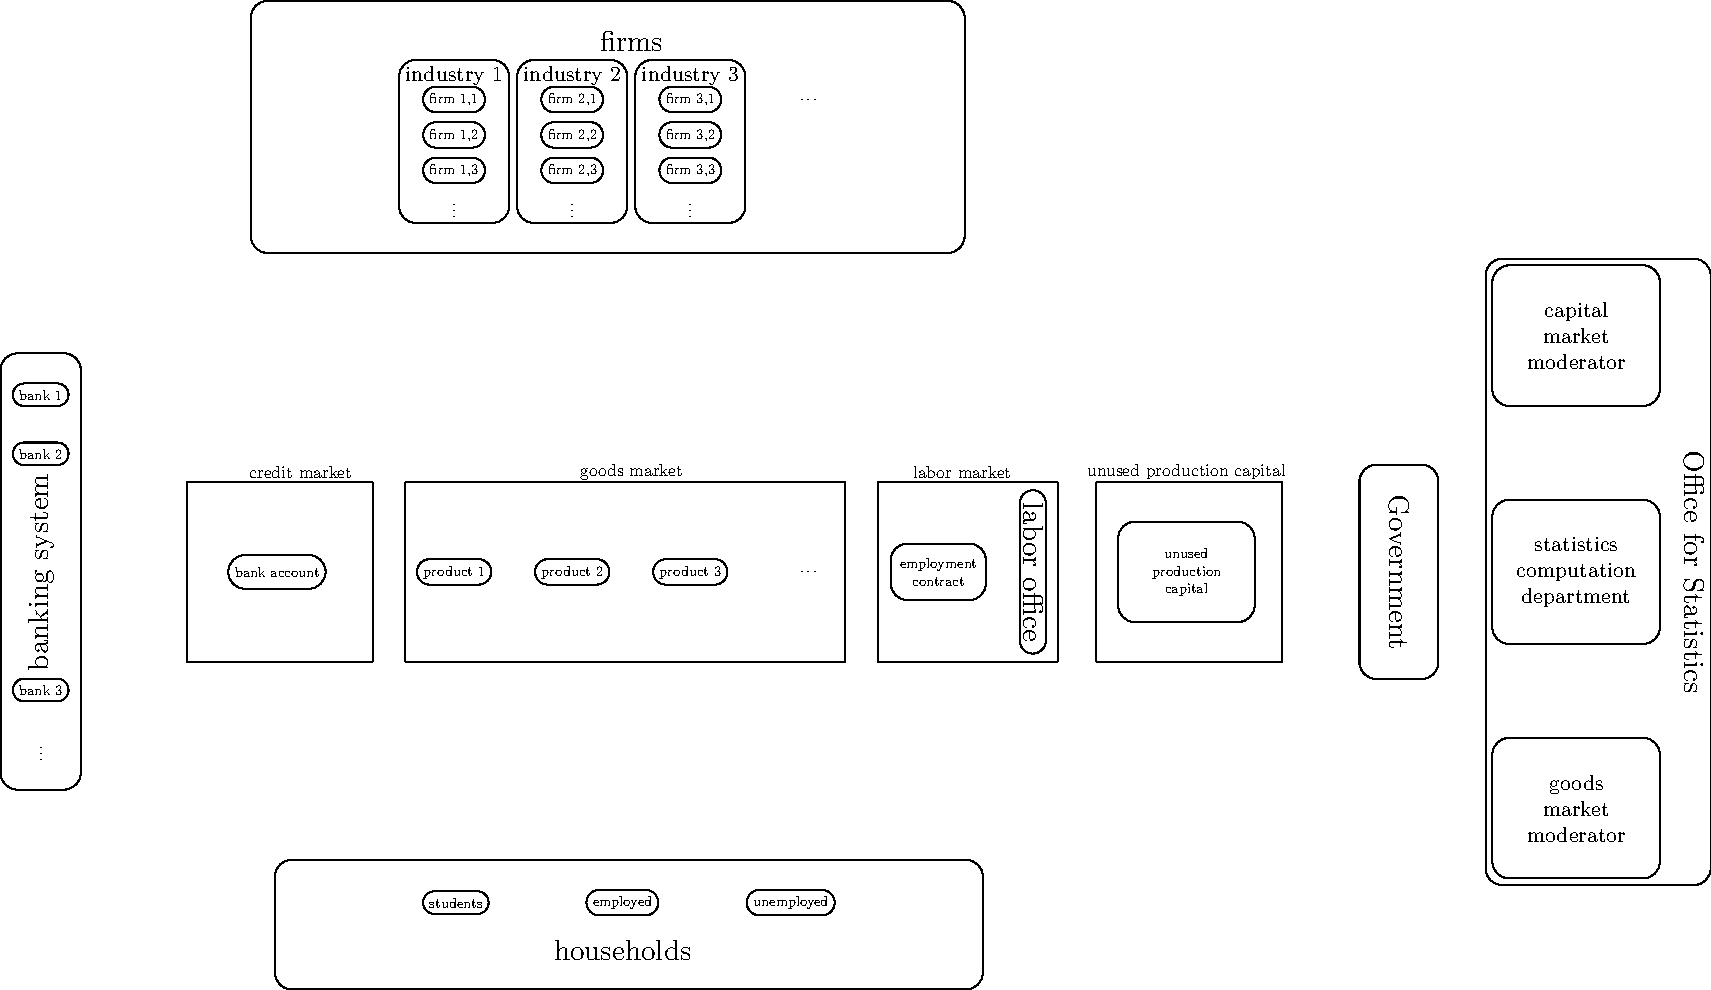
\includegraphics[scale=0.5]{agents_and_interactions_figure1.pdf}
	\caption{Components of the economic system}
	\label{fig:components}
\end{figure}

\begin{figure}[htp]
	\centering
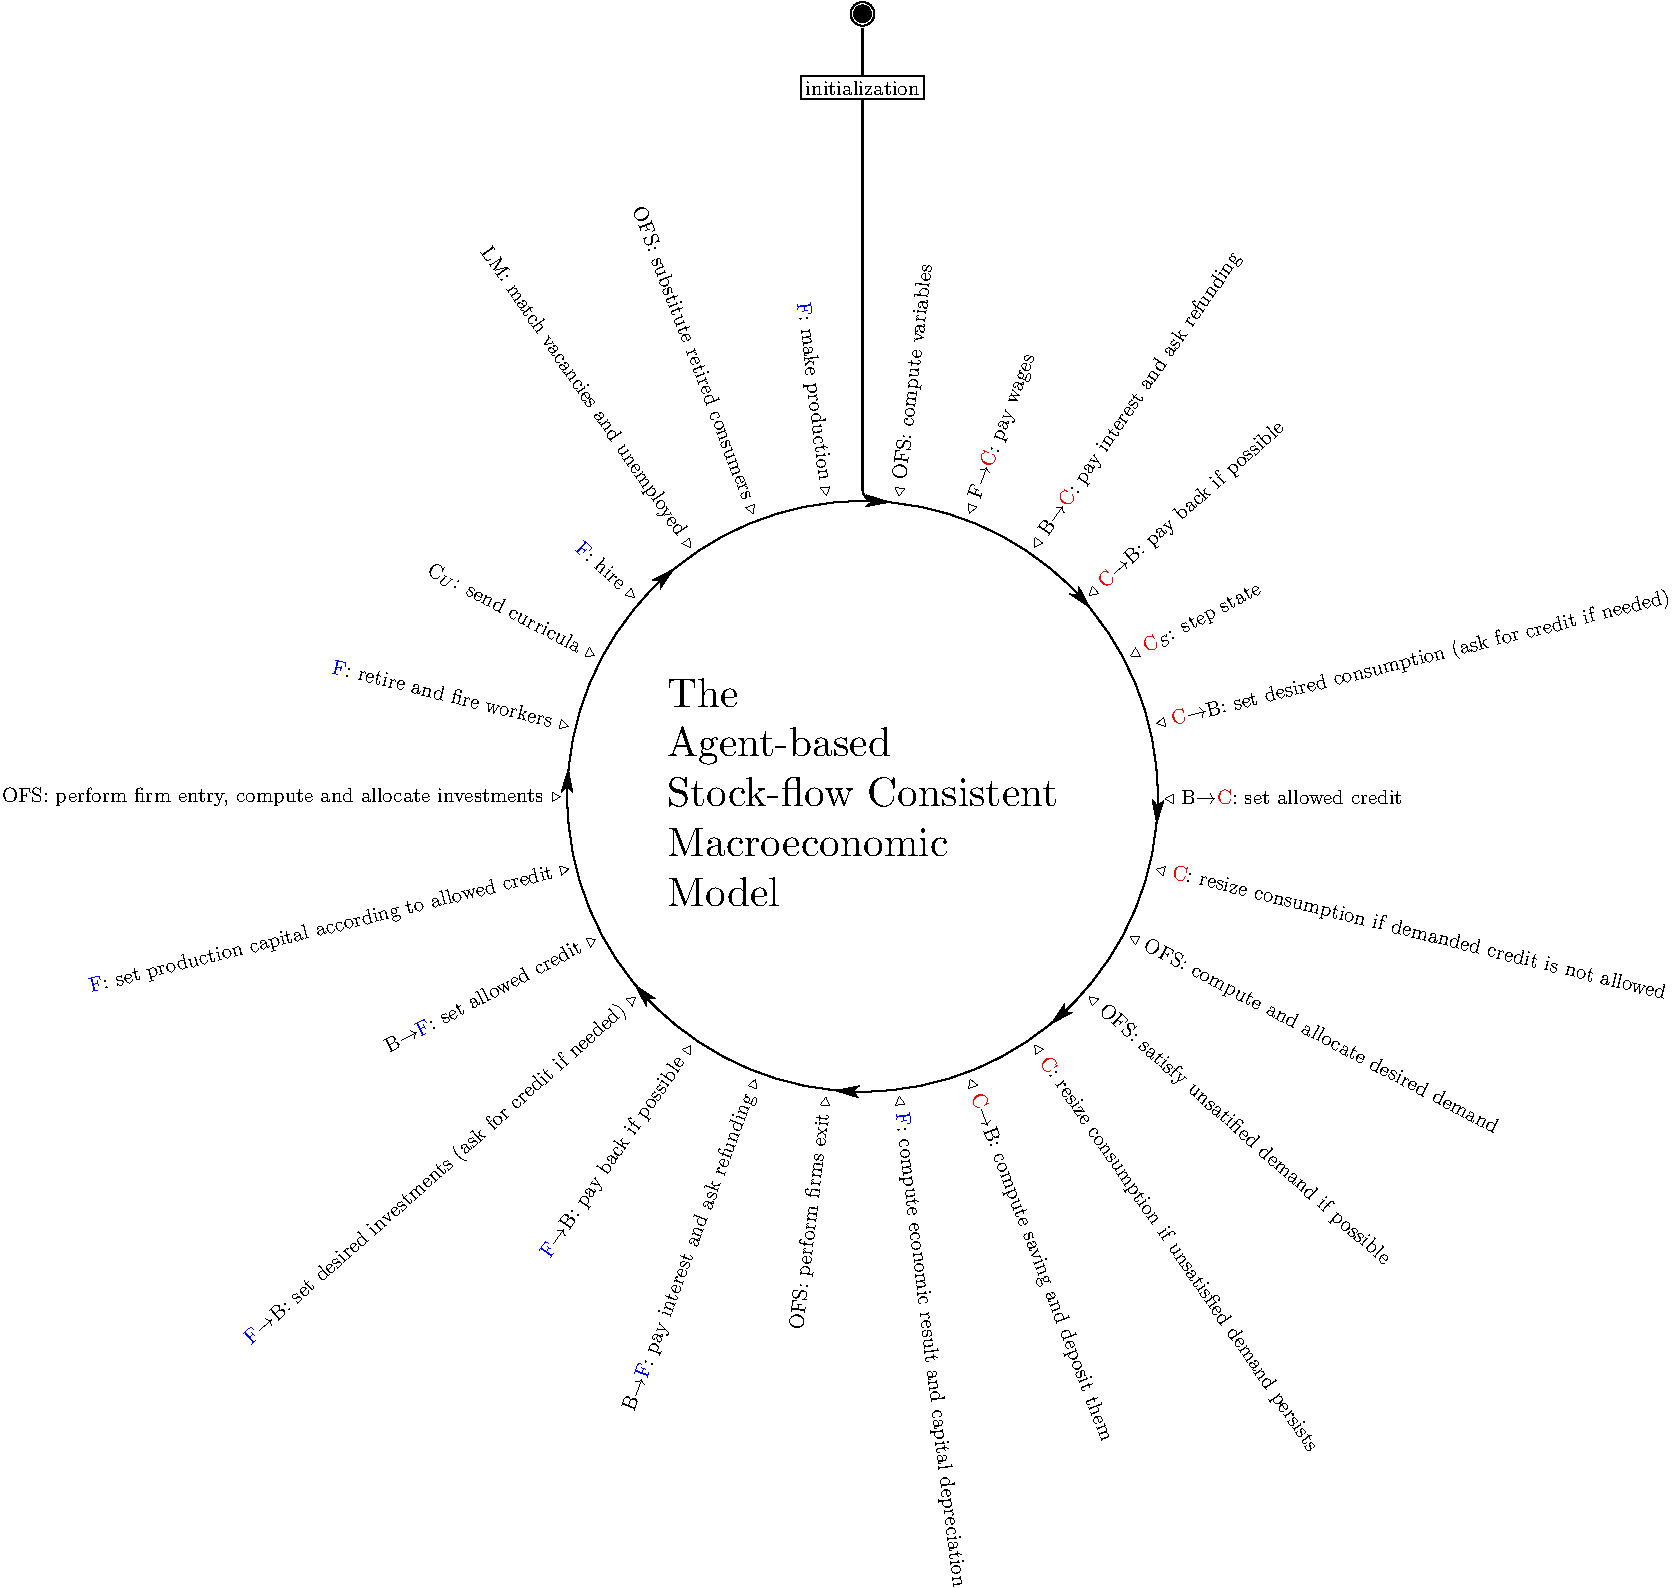
\includegraphics[scale=0.5]{visual.pdf}
	\caption{sequence of events}
	\label{fig:sequence}
\end{figure}

\newpage
%\subsection{System Components}
We divide systems components in the following categories:
\begin{itemize}
	\item agents;
	\item goods;
	\item financial assets.
\end{itemize}
\subsection{Agents}
The characterization of agents is that which is standard in economic modeling:
\begin{itemize}
	\item consumers
	\item firms
	\item government
	\item the banking sector

		$f\in \{1, 2, \cdots, F\}$

\end{itemize}
Beside these agents we have an additional agent that have a global view of the system. It computes aggregate variables, and using this information it supervises the functioning of the models regulating markets and revising agents' individual variables where needed. We call this ``supervisor'' the Office for Statistics.

\subsection{Goods}
\begin{itemize}
	\item consumption goods
	\item investment goods
\end{itemize}

Goods are exchanged on markets.

\subsection{Financial assets}

In the previous section we have identified the type of goods present in our model. The identification and specification of financial products to be included in the model has the same importance and is performed in this section. This task is not trivial and we perform it by using  
%A characteristic of our model is the focus on the coherence at the stock level.
%This push us to use 
a stocks matrix approach that allows us to identify the type of financial assets needed to have a consistent framework. 

As we will explain later on in this section, using this approach we can also identify mechanisms to manage coherently situations of financial stress. The latter are important to study the functioning of the economy in pathological cases.  

To avoid inaccuracies in performing this thorny task, we start from a trivial representation where consumers and firms are present. We then gradually enrich the framework to obtain a configuration where government and banking sectors are also considered.

Before starting we recall that the stock matrix we will use hereafter reports the balance sheets of economic agents. 
Stock consistency implies that the sum of elements in each column and row of the matrix is zero.  


%Before progressing we present the simplest example. 
Let's consider an island-barter economy (money does not exist) populated by a single agent named Robinson Crusoe, whose main activity is to find food. 
The food in the island is perishable and inventories cannot be carried to the following periods. To perform his activity, Robinson establishes the Crusoe\&co to which he bestows his tools ($K$). From an accounting point of view we can distinguish two subjects: Robinson as a consumer and the Crusoe\&co. The balance sheets of the two subjects in the economy are represented as follows:

\vskip5mm
\begin{center}

\begin{tabular}{r c c}
	& \parbox{1.5cm}{\centerline{firm}} & \\
\hline
real	&$K$	& $+$	\\
(production capital)&		&	\\
\hline
financial&$EF$	&$-$	\\
\hline
&$\sum$		&0\\
\end{tabular}


\hskip1cm
\begin{tabular}{r c c }
	
	&household&\\
\hline
financial&$EF$	&	$+$  \\
\hline
counterbalance to financial &$WH$	&$-$\\
(wealth) &	&\\
\hline
&$\sum$	&	0
\end{tabular}


\end{center}
\vskip5mm
note that setting up an accounting framework creates two ``artificial'' categories: the counterpart to the production capital in Crusoe\&co balance sheet, $EF$, that we will call equity capital and the counterpart to equity capital in Robinson's balance sheet, $WH$, that measures his wealth. The signs are used to specify whether the component of the balance sheet is an asset $+$, or a liability $-$.

This reasoning allows us to identify a first category of financial assets: equity capital that %represents the value of $K$; 
in modern economies materializes in \textit{shares}.
With a change of perspective we say that both $K$ and $WH$ counterbalance the financial aspect so that the balance sheet of the two subjects can be summarized in the following stock matrix:

\vskip5mm
\begin{center}

\begin{tabular}{r c c}
	\hline
	& household 	& \parbox{1.5cm}{\centerline{firm}} \\
\hline
\hline
$EF$	&	$+$	&$-$	\\
	\hline
counterbalance to financial	&	$WH$	&$K$	\\
\hline
\hline
$\sum$		&0&0\\
\end{tabular}
\end{center}
\vskip5mm


It is worth emphasizing that the rows of the matrix relate to the types of assets that are accounted for in the economy.  In the simple case presented in this section, we consider only shares as financial assets.

\vskip5mm

As stated above, stock consistency implies that the rows of the matrix also sum to zero:

\vskip5mm
\begin{center}
\begin{tabular}{r c c c}
	\hline
	& household 	& \parbox{1.5cm}{\centerline{firm}}  &$\sum$\\
\hline
\hline
$EF$	&	$+$	&$-$	&0\\
	\hline
counterbalance to financial	&	$WH$	&$K$	&0\\
	\hline
	\hline
$\sum$ &	0	&0	&0
\end{tabular}

\end{center}
\vskip5mm

Let's consider a richer (and more populated) economy where someone invented a new contract. 
The Bank\&co is created to implement a business based on the newly created contract named bank account ($BA$). Both households and firms can sign a bank account contract with the Bank\&co.
 Households, firms and bank can be either lenders or borrowers. The lender records the $BA$ amount with a positive sign while the borrower with a negative sign. Note that the $BA$ amounts are usually referred to as either \textit{deposit}, if the household or the firm act as lenders, or \textit{loan} if they act as borrowers.  

Introducing this agent (the bank), two new financial activities are to be considered in the economy: its equity ($EB$) and the bank account. 
Concerning the latter, instead of using two different rows, one for deposits and one for loans, we think it is more coherent to use one line because the $BA$ is the unique contract an agent can sign with banks. This is of convenience because we will deal with a dynamic context in which a bank account changes its sign from period to period so that considering one entry rather than two will make the accounting easier.   

After considering the $BA$, the agents' balance sheets are:

\vskip5mm
\begin{center}

	\begin{tabular}{r c c }
	
		&\multicolumn{2}{c}{household}\\
\hline
&$BA$	&	$+/-$  \\
&$EB$	&	+  \\
&$EF$	&	+  \\
\hline
counterpart to fin. &$WH$	&$-$\\
\hline
&$\sum$	&	0
\end{tabular}
\hskip5mm
\begin{tabular}{r c c}
	& \multicolumn{2}{c}{firm} \\
\hline
&$BA$	&	$+/-$  \\
&$EB$	&	+  \\
&$EF$	&$-$	\\
\hline
counterpart to fin.	&$K$	& +	\\
\hline
&$\sum$		&0\\
\end{tabular}
\hskip5mm
\begin{tabular}{r c c}
	& \multicolumn{2}{c}{bank} \\
\hline
&$\sum BA$	&	$+$  \\
&$EB$	&	$-$  \\
&$EF$	&$+$	\\
\hline
counterpart to fin.	&	& 0	\\
\hline
&$\sum$		&0\\
\end{tabular}

\end{center}
\vskip5mm

Let us now build a stock matrix for an economy populated by one household, one firm and one bank. We consider the case in which $BA_h>0$, $BA_f<0$ and $BA_h>-BA_f$ and shares are held exclusively by households. The stock matrix is reported in table \ref{tab:sm1}.

\begin{table}
	\centering
\begin{tabular}{r c c c c}
	\hline
	& household 	& \parbox{1.5cm}{\centerline{firm}} & \parbox{1.5cm}{\centerline{bank}} &$\sum$\\
\hline
\hline
$BA$	&	$+$	&$-$	&$BA_h+BA_f$&0\\
$EB$	&	$+$	&	&$-$&0\\
$EF$	&	$+$	&$-$	&&0\\
	\hline
counterbalance to financial	&	$WH$	&$K$	&0\\
	\hline
	\hline
$\sum$ &	0	&0	&0
\end{tabular}
	\caption{stock matrix with $BA_h>0$, $BA_f<0$, $BA_h>-BA_f$ and shares are held exclusively by households}
	\label{tab:sm1}
\end{table}



A visual representation of the matrix is given in figure \ref{fig:vstock0}.
\begin{figure}[htp]
	\centering
\hskip-1cm
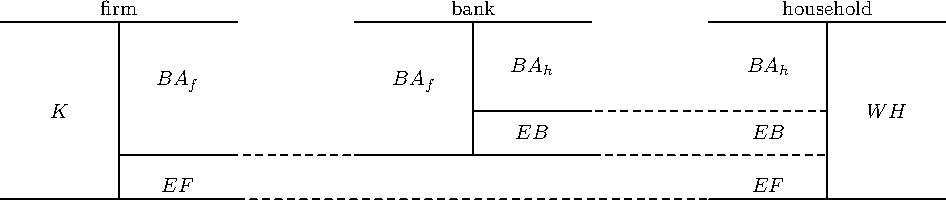
\includegraphics[scale=0.8]{balances-0.pdf}
	\caption{visual representation of the stock matrix}
	\label{fig:vstock0}
\end{figure}
It shows the result often highlighted in macroeconomic textbook that in this kind of economy, wealth equates production capital:
\[WH=K\]
but it also shows less straightforward relationships such as 
\[
	 K=BA_h+EB+EF
\]
or
\[
W=BA_f+EF
\]
A slightly more sophisticated case in obtained by letting banks and firm holding each other shares. The stock matrix is now reported in table \ref{tab:sm2} and visually represented in figure \ref{fig:vstock1}.

\begin{table}[t]
	\centering
\begin{tabular}{r c c c c}
	\hline
	& household 	& \parbox{1.5cm}{\centerline{firm}} & \parbox{1.5cm}{\centerline{bank}} &$\sum$\\
\hline
\hline
$BA$	&	$+$	&$-$	&$BA_h+BA_f$&0\\
$EB$	&	$+$	&$+$	&$-$&0\\
$EF$	&	$+$	&$-$	&$+$&0\\
	\hline
counterbalance to financial	&	$WH$	&$K$	&0\\
	\hline
	\hline
$\sum$ &	0	&0	&0
\end{tabular}
	\caption{stock matrix with $BA_h>0$, $BA_f<0$, $BA_h>-BA_f$ and shares are held by all the agents}
	\label{tab:sm2}
\end{table}

\begin{figure}[t]
	\centering
\hskip-1cm
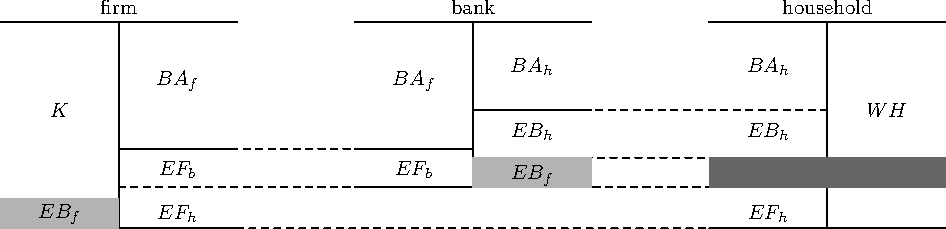
\includegraphics[scale=0.8]{balances-1.pdf}
	\caption{visual representation of the stock matrix}
	\label{fig:vstock1}
\end{figure}
The figure shows some gray area. They are introduced to find our relationships among balance sheet variables by visual inspection. In particular, the darker gray area signal areas that have to be discarded from the considered balance sheet while lighter ones are balance sheet items that are important for deducing relationships.  Consider for example firm assets. Their amount is given by
\[K+EB_{f}\]
looking now to household's liabilities we deduce that we have to add the dark gray area to wealth to reach the same amount of firm assets. But the dark gray area is equal to $EB_{f}$. So we can write
\[K+EB_{f}=WH+EB_{f}\]
that brings us to state that
\[WH=K\]
holds again. 
%In fact, to obtain the household's balance sheet we hat to remove the gray area. Its amount is equal to equity issued by the bank and hold by the firm ($E_{b,f}$). This is the same amount one have to subtract from the firm assets to obtain the production capital, thus $K=W$. 
As we did above, we can specify less straightforward relationships such as
\[K=BA_h+EB_{h}+EF_{h}\]
\[
	WH=BA_f+EF_{h}+(EF_{b}-EB_{f})
\]
that generalizes what written above.

We can now complete our framework by introducing the government. This also introduces an additional financial asset: government bonds ($GB$). 
Table \ref{tab:bsall} reports the balance sheets, table \ref{tab:sm3} the stock matrix and figure \ref{fig:vstock2} the visual representation of the new situation. 
We can again deduce the economic equations.
\[W+EB_{f}-GB_{f}=K+GB_b+GB_f+EB_{f}\]
\[WH=K+GB_b+GB_f+GB_{f}\]
\[WH=K+WG\]


\begin{table}[p]
	\begin{center}

	\begin{tabular}{r c c }
	
		&\multicolumn{2}{c}{household}\\
\hline
&$BA$	&	$+/-$  \\
&$EB$	&	+  \\
&$EF$	&	+  \\
&$GB$	&	+  \\
\hline
counterpart to fin. &$WH$	&$-$\\
\hline
&$\sum$	&	0
\end{tabular}
\hskip5mm
\begin{tabular}{r c c}
	& \multicolumn{2}{c}{firm} \\
\hline
&$BA$	&	$+/-$  \\
&$EB$	&	+  \\
&$GB$	&$+$	\\
&$EF$	&$-$	\\
\hline
counterpart to fin.	&$K$	& +	\\
\hline
&$\sum$		&0\\
\end{tabular}
\hskip5mm
\begin{tabular}{r c c}
	& \multicolumn{2}{c}{bank} \\
\hline
&$\sum BA$	&	$+$  \\
&$GB$	&	$+$  \\
&$EB$	&	$-$  \\
&$EF$	&$+$	\\
\hline
counterpart to fin.	&	& 0	\\
\hline
&$\sum$		&0\\
\end{tabular}
\hskip5mm
\begin{tabular}{r c c}
	& \multicolumn{2}{c}{government} \\
\hline
&$\sum GB$	&	$-$  \\
\hline
counterpart to fin.	&$WG$	& +	\\
\hline
&$\sum$		&0\\
\end{tabular}


\end{center}
	\caption{balance sheets with government bonds}
	\label{tab:bsall}
\end{table}



\begin{table}[p]
	\centering
\begin{tabular}{r c c c c c}
	\hline
	& household 	& \parbox{1.5cm}{\centerline{firm}} & \parbox{1.5cm}{\centerline{bank}} & \parbox{1.5cm}{\centerline{gov}} &$\sum$\\
\hline
\hline
$BA$	&	$+$	&$-$	&$BA_h+BA_f$&&0\\
$EB$	&	$+$	&$+$	&$-$&&0\\
$EF$	&	$+$	&$-$	&$+$&&0\\
$GB$	&	$+$	&$+$	&$+$&$-$&0\\
	\hline
counterpart	&	$WH$	&$K$&0&$WG$	&0\\
	\hline
	\hline
$\sum$ &	0	&0	&0&0
\end{tabular}
	\caption{stock matrix with $BA_h>0$, $BA_f<0$, $BA_h>-BA_f$ and shares are held by all the agents}
	\label{tab:sm3}
\end{table}

\begin{figure}[p]
\hskip-3cm
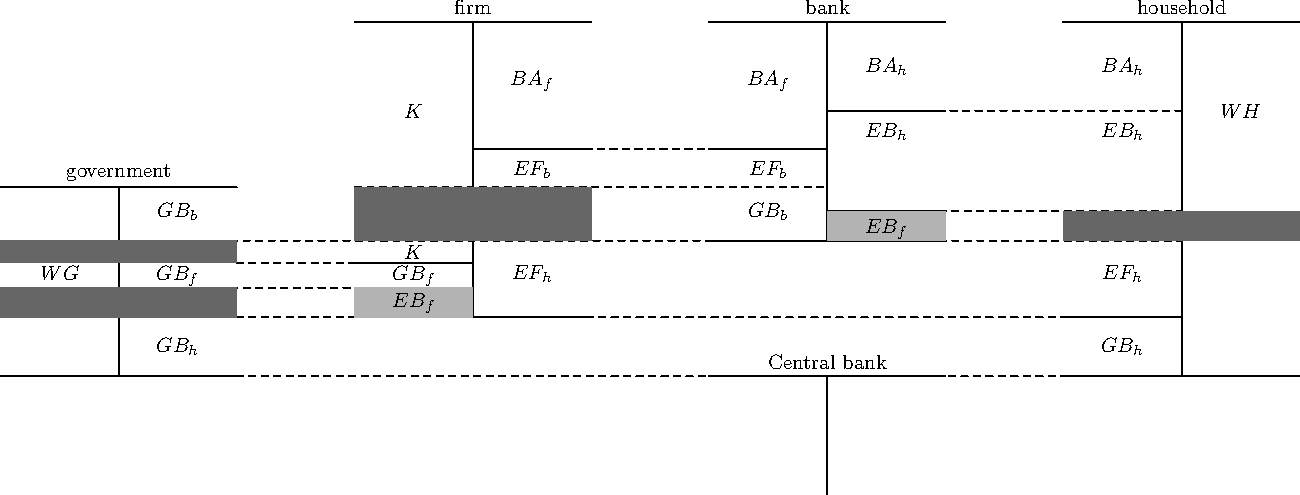
\includegraphics[scale=0.8]{balances-2.pdf}
	\caption{visual representation of the stock matrix}
	\label{fig:vstock2}
\end{figure}

\clearpage


Figure \ref{fig:vstock2} presents a rather complicate situation. We now simplify it to reach a starting point for considering situation of agents' financial stress. 
%We proceed by making two simplifications that brings us to our initial situation where shares are hold exclusively by households. 
The simplifications is: shares abd bonds are hold exclusively by households. 

Figure \ref{fig:vstock5} shows the simplified situation.   

\iffalse
\begin{itemize}
	\item the firm do not possesses bank shares
	\item the firm do not possesses government bonds
	\item the bank do not possesses the firm shares
\end{itemize}

represented in figures \ref{fig:vstock3} and \ref{fig:vstock4}.
Figure \ref{fig:vstock4} shows the simplified situation.   


\begin{figure}[p]
\hskip-3cm
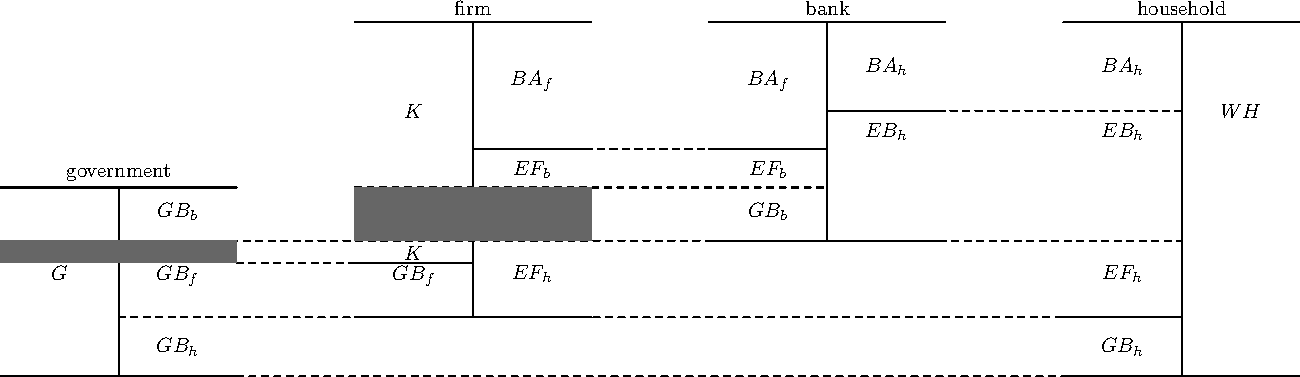
\includegraphics[scale=0.8]{balances-3.pdf}
	\caption{visual representation of the stock matrix}
	\label{fig:vstock3}
\end{figure}

\begin{figure}[ht]
\hskip-3cm
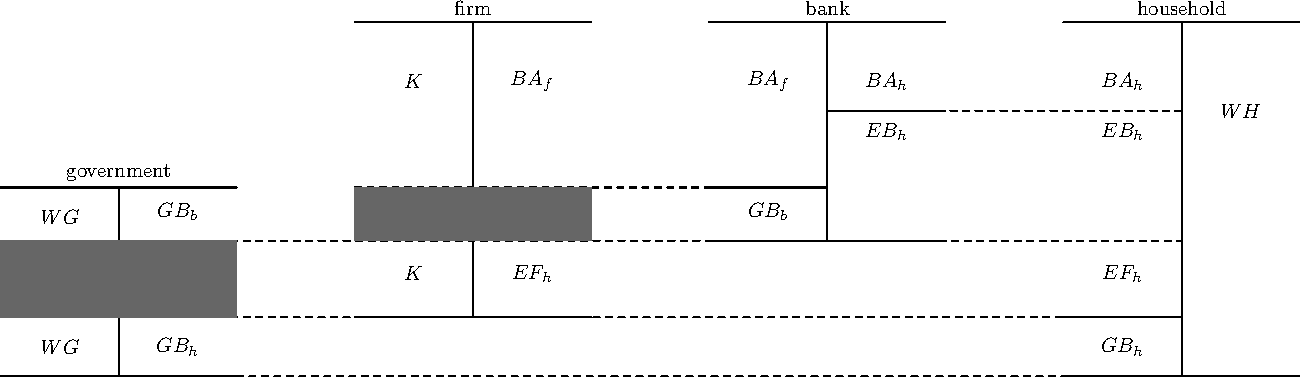
\includegraphics[scale=0.8]{balances-4.pdf}
	\caption{visual representation of the stock matrix}
	\label{fig:vstock4}
\end{figure}
\fi

\begin{figure}[ht]
\hskip-3cm
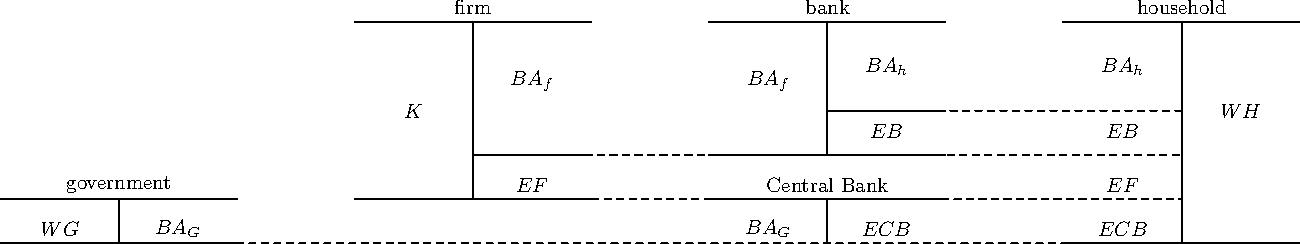
\includegraphics[scale=0.8]{balances-5.pdf}
	\caption{visual representation of the stock matrix}
	\label{fig:vstock5}
\end{figure}



\clearpage
The aggregate stock matrix is obtained by summing over individual values and is reported in table \ref{table:simplified}.

%\vskip5mm
\begin{table}[htp]
\begin{center}
\begin{tabular}{l c c c c c}
	\hline
&	& Household 	& \parbox{1.5cm}{\centerline{Firm}}   & \parbox{1.5cm}{\centerline{Bank}} &$\sum$\\
\hline
\hline
$BA$	&	&$\sum_h BA$	&$\sum_f BA$	&$-\sum_b (\sum_h BA+\sum_f BA)$	&0\\
$E_f$	&	&$\sum_h E_f$	&-$\sum_f E_f$	&$\sum_b E_f$	&0\\
$E_b$	&	&$\sum_h E_b$	&$\sum_f E_b$	&-$\sum_b E_b$	&0\\
	\hline
counterbalance	&&		&	&	&\\
to financial	&&	$\sum_hW$	&$\sum_fK$	&0	&0\\
assets	&&		&	&	&\\
	\hline
	\hline
&$\sum$	&	0	&0	&0	&0\\
\end{tabular}
\end{center}
\caption{A simplified bottom-up stock matrix with a banking sector}
\label{table:simplified}
\end{table}



In each balance sheet, one variable is determined as the complement to the others:

\[
W_h=BA_h+E_b+E_f
\]
\[
E_f=K_f-BA_f+E_b
\]
\[
E_b=\sum BA+E_f
\]

Economic models usually account for the ``normal'' case in which the three variables reported above have positive values. However, it is worth considering ``pathological'' cases in which these variables get negative. This section shed light on how these cases should be treated.  

\newpage 
\newpage
\section{Initialization}
The initialization phase aims allowing firms to determine their initial production reducing exogenous setting to the minimum. 

When the production is computed, the sequence of events can progress by entering the main loop. During the initialization process, the stock variables of all agents will be set in a stock flow consistent way.

We will describe the initialization process in a more detailed way hereafter.

To realize production firms need two production input: capital and labor. We use the following Leontief type production function:
\[
Y_f=\min(Y_f^{PK},Y_f^{PL})
\]
That is, production realized by firm $f$ is the minimum between the firm potential production capital production, $Y_f^{PK}$, and the potential production that can be obtained by the labor force employed by the firm, $Y_f^{PL}$. 


The capital potential production is assumed to be equal to the level of capital:
\[
	Y^{PK}_f=K_f
\]

The potential production of labor is more tricky because workers are heterogeneous and has different productivities.
If we identify a worker's productivity with $wp_{w,f}$, we compute the sum of workers productivities
\[
	wp_f=\sum_{w}wp_{w,f}
\]
the potential production is thus
\[
	Y^{PL}_f=\theta_{YL}wp_f
\]
parameter:\\
\begin{tabular}{l l l}
	\hline
	in papers& in code&value\\
	\hline
	\hline
$\theta_{YL}$&\verb+parameterOfProductivityInProductionFuncion+&100\\
	\hline
\end{tabular}

\vskip5mm
To arrive at the very first $Y_f$ we adopt the following strategy. 
\begin{itemize}
	\item compute the potential output from workers
	\item adjust capital such as the potential output from capital is equal to the potential output from workers 
\end{itemize}

Note how the first step implies a preliminary setup of consumer state, while the second step allows the setup of firms assets balance sheet item. 
Following the second step, we can setup firms balance sheet liabilities.
Once consumers and firms banks accounts are known, we setup banks balance sheets.

So the whole initialization sequence has the following phases:
\begin{enumerate}
	\item Create agents
	\item set consumers working state
	\item set agents balance sheet
	\item revise agents balance sheet for stock consistency
\end{enumerate}

We will now discuss the initialization for each type of agent.

\subsection{Consumers initialization}

\subsubsection{Working situation}


\subsubsection*{Students}

In an attempt to reduce the number of parameters to the minimum, it is assumed that each worker is characterized by its fundamental ability. It characterize each consumer performance during the education period. The latter in turn determine the productivity as a worker.

We call this parameter the student ability.\\
parameters:\\
\begin{tabular}{l l l}
	\hline
	in papers& in code&value\\
	\hline
	\hline
$\theta_{as}$&\verb+abilityStudent+&\verb+U(Context.minAbilityStudent,+\\
& &\verb+Context.maxAbilityStudent)+\\
 $\theta_{minas}$&\verb+Context.minAbilityStudent+&$0.35$\\
 $\theta_{maxas}$&\verb+Context.maxAbilityStudent+&$0.5$\\
	\hline
\end{tabular}

\vskip5mm
The most important observation about this parameter is that its upper value is 0.5.

Next important variable is the consumers age, which is initialized as a random number between zero and a parameter denoting the retirement age.\\
parameter:\\
\begin{tabular}{l l l}
	\hline
	in papers& in code&value\\
	\hline
	\hline
 $\theta_{cea}$&\verb+Context.consumerExitAge+&$70$\\
	\hline
\end{tabular}

\vskip5mm
Using the \verb+abilityStudent+ and the \verb+consumerAge+ the education history of consumers is inizialized. Each year of education is set to successful if
\[
	u<2\theta_{as}
\]
and unsuccessful otherwise. $u$ is drawn from a $U(0,1)$. Note that best students has $\theta_{as}=0.5$, so they will be alway successful because $2\theta_{as}=1$. Students with less abilities has lower probability to be successful.\\

To initialize the education history we need the following\\ 
parameters:\\
\begin{tabular}{l l l}
	\hline
	in papers& in code&value\\
	\hline
	\hline
 $\theta_{mnfpe}$&\verb+maxNumberOfFailedPeriodsOfEducation+&$2$\\
 $\theta_{mnpe}$&\verb+maxNumberPeriodsOfEducation+&$21$\\
	\hline
\end{tabular}

\vskip5mm
Starting from age 0, the process is repeated until 
\begin{enumerate}
	\item the maximum number of failures admitted ($\theta_{mnfpe}$) or
	\item the maximum periods of possible education ($\theta_{mnpe}+\theta_{mnfpe}$) or
	\item the consumer's age 
\end{enumerate}
is reached.

We then count the number of successful periods of education, $n_{sye}$. 

When the process is stopped by conditions 1 or 2, the consumer state is set to non students. At this stage, all non students are unemployed. This state will be revised in the next step. Both the education degree and the productivity as a worker are assigned using $n_{sye}$. 

The degree of education is assigned as follows:
\[
	\begin{array}{l l l}
		n_{sye}& \textnormal{degree}& \textnormal{degree id}\\
	0\le n_{sye}<5 & \textnormal{none}&0\\
	5\le n_{sye}<8 & \textnormal{elementary}&1\\
	8\le n_{sye}<13 & \textnormal{intermediate}&2\\
	13\le n_{sye}<16 & \textnormal{college}&3\\
	16\le n_{sye}<18 & \textnormal{bachelor}&4\\
	18\le n_{sye}<21 & \textnormal{master}&5\\
	21= n_{sye} & \textnormal{PhD degree}&6
	\end{array}
\]

The productivity is assigned as follows. Each year of education increases the consumers ability by a fixed amount. So, the productivity assigned to a non worker with  $n_{sye}$ successful year of education is
\[
	wp=\theta_{as}+\frac{0.5}{\theta_{mnpe}}n_{sye}
\]
Note that $\theta_{as}=0.5$ implies $n_{sye}=\theta_{mnpe}$ so that $wp=1$.

Once the productivity of a non student is known, we compute his/her potential production 
\[Y^{Pns}=\theta_{YL}wp\]

The education history initialization is stopped by condition 3 when the consumer is young. In this case the subject is assigned the state of student and its education history will be evolved in the main loop using the rules explained above.

\subsubsection*{Employed and unemployed}

At this stage all non students are unemployed. Now, some of them will be employed by firms. 

To perform this task we introduce the following\\
parameter:\\
\begin{tabular}{l l l}
	\hline
	in papers& in code&value\\
	\hline
	\hline
 $\theta_{ptbub}$&\verb+Context.probabilityToBeUnemployedAtTheBeginning+&$0.2$\\
	\hline
\end{tabular}

\vskip5mm
With probability $1-\theta_{ptbub}$, each non student select a firm randomly and send his/her CV to this firm. Subjects who do not send a CV (this happens with probability $\theta_{ptbub}$) enter the main loop in the unemployments state. 

\subsubsection{Proposing consumers bank account}

This is a first action to setup the consumers balance sheet. 

The involved parameters are:\\
\begin{tabular}{l l l}
	\hline
	in papers& in code&value\\
	\hline
	\hline
 $\theta_{nbcc}$&\verb+Context.numberOfBanksAConsumerCanBeCustumerOf+&$1$\\
 $\theta_{mincba}$&\verb+Context.minConsumerInitialBankAccount+&$-500$\\
 $\theta_{maxcba}$&\verb+Context.maxConsumerInitialBankAccount+&$500$\\
	\hline
\end{tabular}

\vskip5mm

Each consumer select randomly a number of banks equal to $\theta_{nbcc}$ and open a bank account in each of them. To set the amount of the bank account the code drawn a random integer from a uniform distribution $U(\theta_{mincba},\theta_{maxcba})$. In case the figure is negative the amount is set to zero and the drawn number is assigned to the demandedCredit variable (it will managed when the bank account will be setup). Non negative number are assigner to the bank account amount.

The amount will be revised in the final step of the initialization to ensure stock consistency.

\subsection{Firms initialization}
\subsubsection{Potential production of labor}
In the consumers initialization we saw that some non student sent their CV to firms.

Each Firm now has a list of CVs. Each firm employs all the senders of the CVs that are in the received CVs list. The CV senders state is switched from unemployed to employed.

Summing the potential production of each employee, the firm determine the potential production of its labor force:
\[
	wp_f=\sum_{w}wp_{w,f}
\]
the potential production is thus
\[
	Y^{PL}_f=\theta_{YL}wp_f
\]

\subsubsection{Production capital}
As we told above, due to the Leontif production function, the production capital is set in such a way that the potential production from capital is equal to the potential production of labor. We have already defined the potential production of capital as
\[Y_f^{PK}=K_f\]
So, the initial level of capital for each firm is set to
\[
K_f=Y^{PL}_f
\]
\subsubsection{Balance sheet}

In the previous step we set up the assets side of the firms balance sheet.

As explained above, we have two liabilities: equity and bank account. We set up equity and determine the bank account residually.

To setup equity we need these\\
parameters:\\
\begin{tabular}{l l l}
	\hline
	in papers& in code&value\\
	\hline
	\hline
 $\theta_{minfieb}$&\verb+Context.minFirmInitialEquityRatio+&$0.1$\\
 $\theta_{maxfieb}$&\verb+Context.maxFirmInitialEquityRatio+&$0.3$\\
	\hline
\end{tabular}

\vskip5mm
Each firm equity is set as follow
\[
	EF_f=u_{Ef}K_f
\]
where $u_{Ef}$ is drawn from $U(\theta_{minfieb},\theta_{maxfieb})$.

Finally, each firm sets her bank accounts. First of all the level of bank account is computed as
\[
BA_f=K_f-EF_f
\]

The model has a parameter for the number of banks a firm can be costumer of\\
parameter:\\
\begin{tabular}{l l l}
	\hline
	in papers& in code&value\\
	\hline
	\hline
 $\theta_{nbbc}$&\verb+Context.numberOfBanksAFirmCanBeCustumerOf+&$1$\\
	\hline
\end{tabular}

\vskip5mm
each firm selects randomly a number of banks equal to $\theta_{nbbc}$ and open a bank account in each of them. The amount of the bank account is set to zero (will be assigned in the next step when the bank balance sheet will be initialized), but the variable demanded credit is each bank account is set to $BA_f/\theta_{nbbc}$.


\subsection{Banks initialization}


To setup the banks balance sheet, we start again from their assets.
The amount of negative bank accounts is summed up. This gives the loans extended a bank:
\[
L_b=\sum BA_b^-
\]



Given each bank assets, we setup the equity by using the following\\
parameters:\\
\begin{tabular}{l l l}
	\hline
	in papers& in code&value\\
	\hline
	\hline
 $\theta_{minbier}$&\verb+Context.minBankInitialEquityRatio+&$0.1$\\
 $\theta_{maxbier}$&\verb+Context.maxBankInitialEquityRatio+&$0.3$\\
	\hline
\end{tabular}

\vskip5mm
A bank equity base of a bank is then computed as
\[
	EB_b=u_{Eb}L_b
\]
where $u_{Eb}$ is drawn from $U(\theta_{minbieb},\theta_{maxbieb})$.

Now, the level of deposits compatible with the balance sheet relationship is computed:
\[
D_b=L_b-EB_b
\]

Due to the random elements in the initialization of consumers and firms, we in general have
\[
	\sum BA^+_b \neq D_b
\]
To satisfy the balance sheet identity, the amount of positive bank accounts is adjusted as follows:
\[
	BA^{+adj}=BA^+\frac{D_b}{\sum BA^+_b}
\]
In this way, stock consistency in each bank balance sheet is restored:
\[
	\sum BA^{+adj}_b=D_b
\]

\newpage
\section{The main loop}
The main loop can be divided into two parts:
\begin{enumerate}
	\item the process that leads to the production of goods
	\item the process that leads to the consumption of what has been produced
\end{enumerate}

\begin{figure}[htp]
	\centering
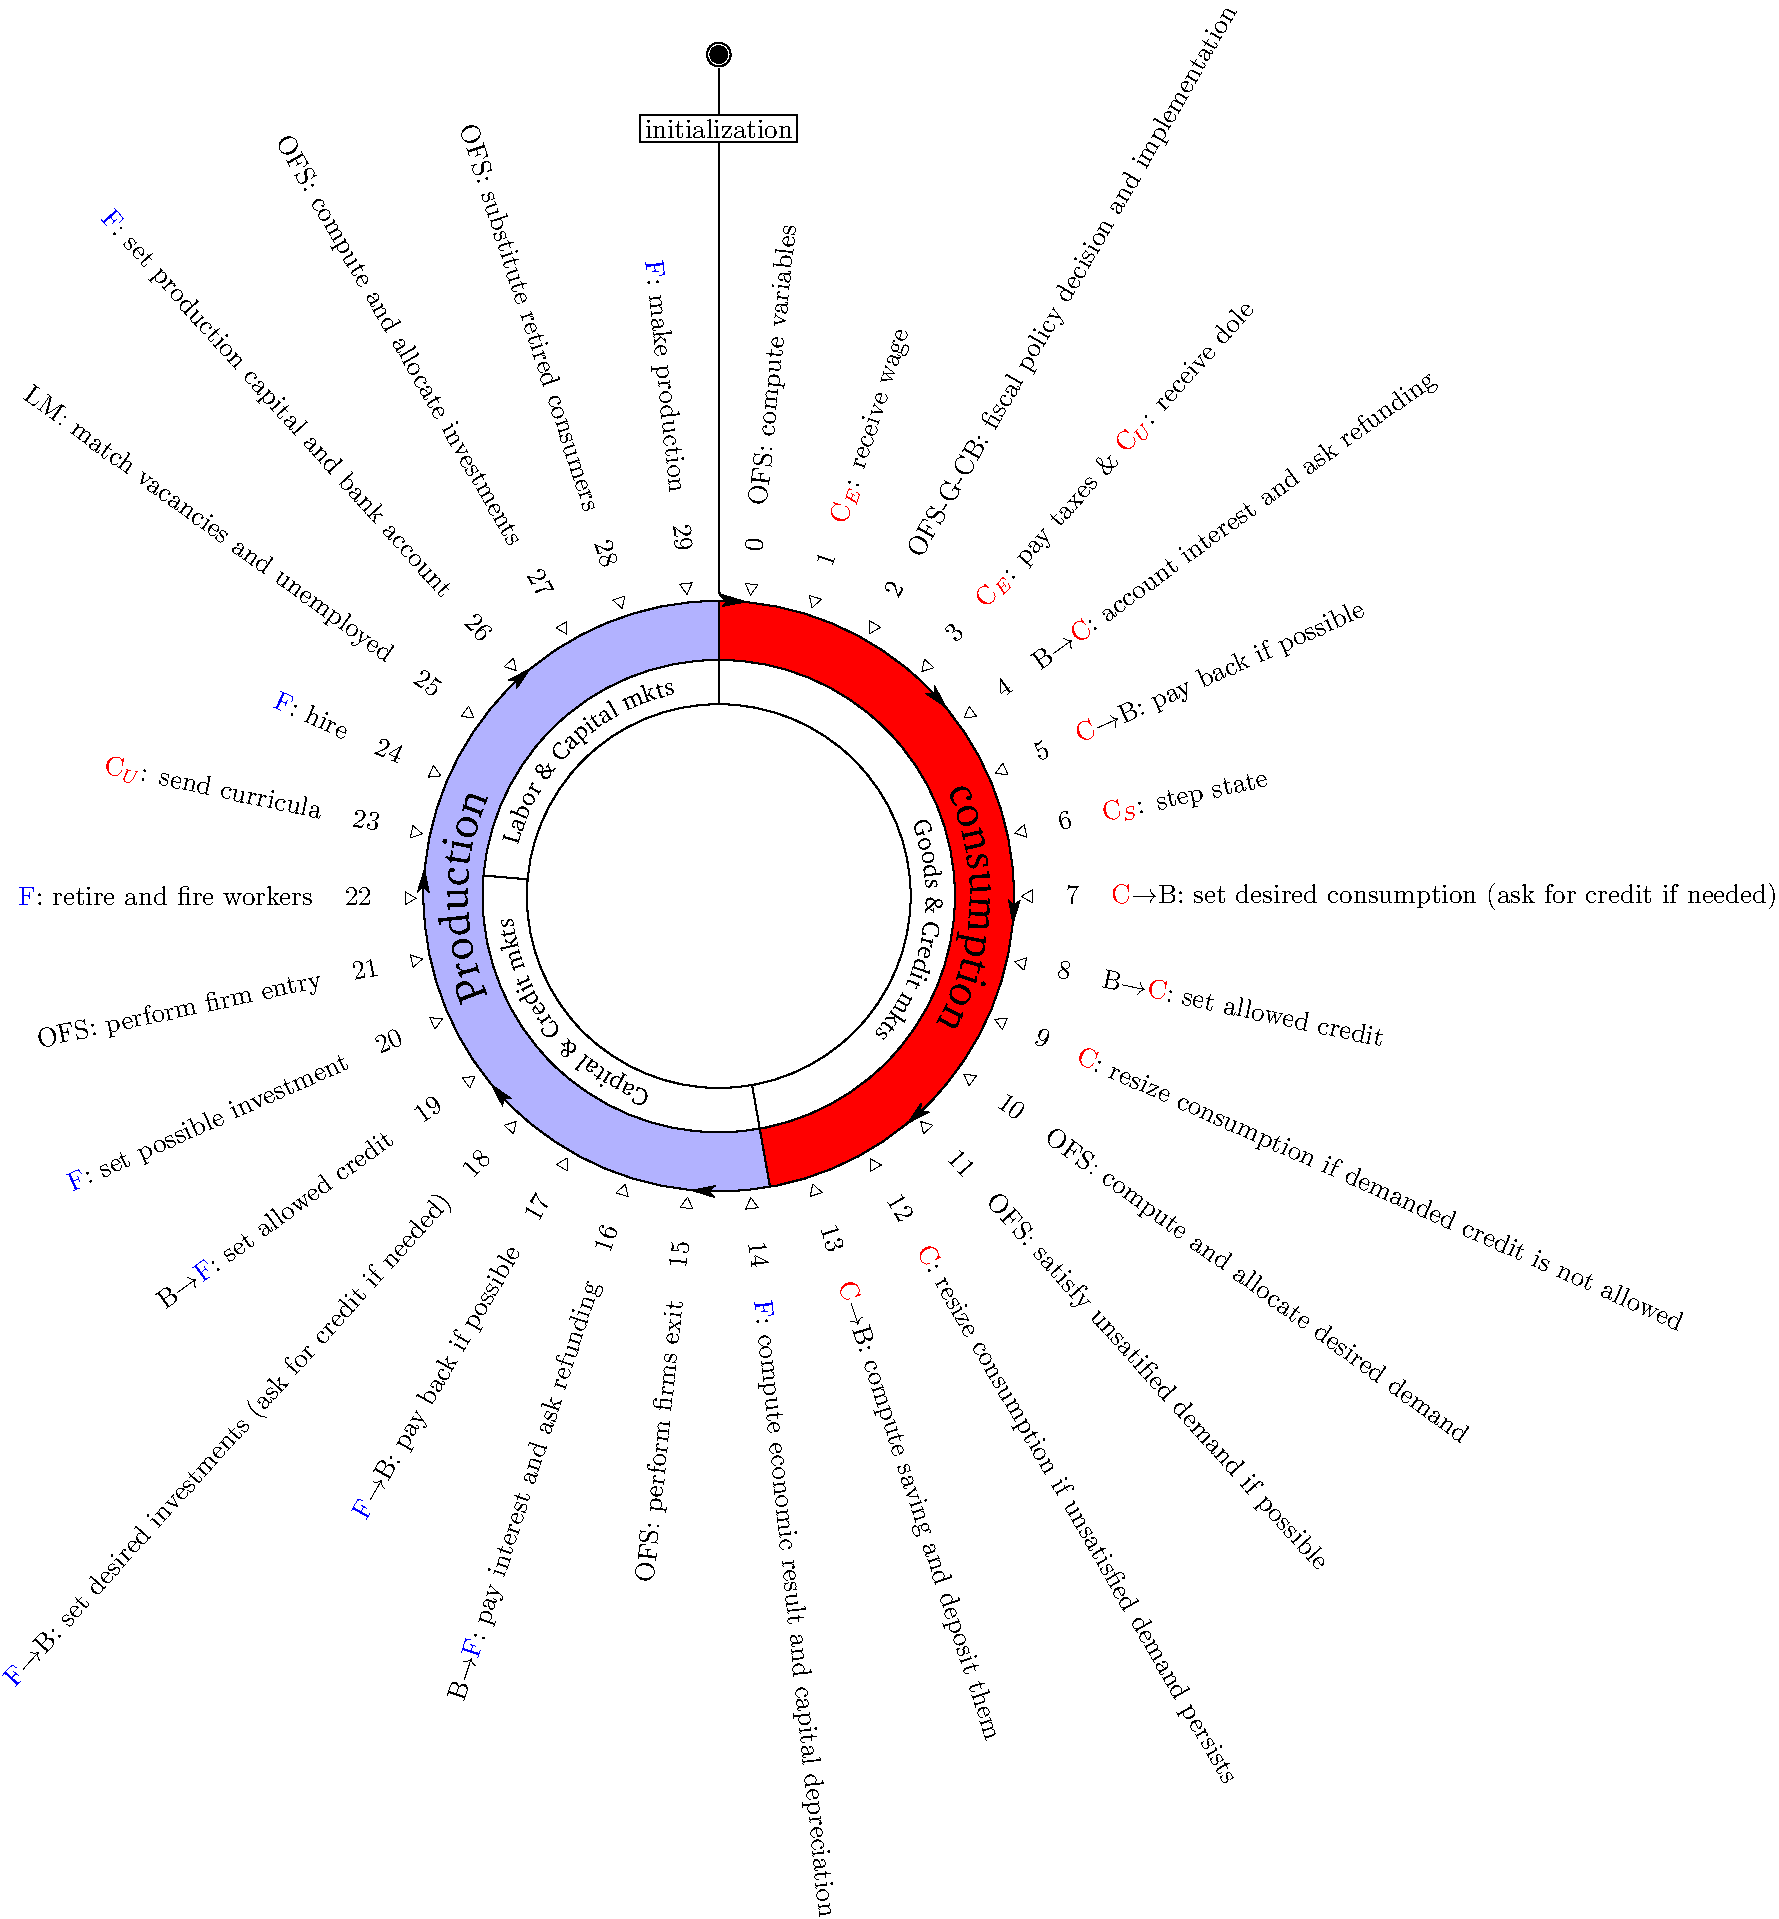
\includegraphics[scale=0.5]{visual1.pdf}
	\caption{sequence of events}
	\label{fig:clockcolor}
\end{figure}

\subsection{the process that leads to the consumption of what has been produced}
%\subsection{Consumer-market-bank relationship}
We present here the sequence of events and will enter in the details in the following subsections.

\begin{enumerate}
	\item consumers receive wages;
	\item banks 
		\begin{enumerate}
			\item account interest
			\item ask for loan repayments to indebted consumers;
		\end{enumerate}
	\item consumers refund if possible (if they have enough financial resources);
	\item students update their state
	\item consumers 
		\begin{enumerate}
			\item compute their desired consumption
			\item compute if they have enough financial resources to realize their desired consumption
			\item if financial resources are needed to realize desired consumption or unpaid amounts exists, consumers check if banks to whom credit can be asked exists and choose the one with the ``best'' bank account;
			\item if financial resources are needed and the best bank account exists, consumers asks for new credit. Credit can be asked to consume more than the available resources and/or to repay outstanding debt that they are able to refund;
		\end{enumerate}
	\item banks decide how much credit to allow;
	\item consumers adjust their desired consumption according to allowed credit. 
	\item Consumers go in the good market in order to satisfy their possible demand.
	\item Office for statistics helps finding goods.
	\item The \textit{effective} level of consumption is established: it may be less or equal to the desired consumption.
	\item consumers adjust their bank accounts (deposits and loans) according to effective consumption.
\end{enumerate}

\subsubsection{Consumer-Bank relationship}

\begin{table}[htp]
	\resizebox{\linewidth}{!}{
\begin{tabular}{c c c c}
	\hline \hline
	 & \multicolumn{2}{c}{\textbf{Traditional modeling}}& \textbf{Additional information}\\
		\hline \hline 
	Step&Flow&Stock&\\
	\hline
	initial	&		&$BA$		&\\
	\hline
	1	&		&		&new about income \\
	\hline
	2a	&$iBA$		&$BA+iBA$	&\\ %questo è giusto per interessi anticipati
%	\hline
	2b	&		&		&$\Delta BA^{db}$ desired by banks\\
	\hline
	3	&	&	&$ref=\min(w-c^s,\Delta BA^{db})$\\
%	\hdashline
	3	&		&		&$unpaid=\Delta BA^{db}-ref$\\
	\hline
	5a	&		&		&desider consumption ($c^d$)\\
%	\hdashline
	 5b&		&		&$\Delta BA^{dc}$ desired by consumers\\
		&		&		&$=\max(0,c^d-(w-ref))+unp$\\
	5c	&		&		&$bestBank=\{identified, not\ exist\}$\\
	5d	&		&		&if bestBank exists ask $\Delta BA^{dc}$ to it \\
	\hline
	6	&		&		&$\Delta BA^{ab}$ allowed by banks\\
%	\hdashline
		&		&		&$\Delta ref=-\Delta unp$\\
%		\hdashline
		&		&		&$\Delta BA^{ab}$ available for consumption\\
%		\hdashline
		&		&		&=$\Delta BA^{ab}-\Delta ref$\\
	\hline
	7	&		&		&$c^{pb}$ consumption possible by credit\\
%	\hdashline
	\hline
	10	&		&		&$c$ consumption possible by market\\
	\hline
%	9	&$\max(w-ref-c,0)$	&$BA+iBA+ref$	&\\
%		&		&	$+\min(w-ref-c,0)$&\\
%		&		&	\\
%		\hdashline
	11	&$w-c$		&	$BA+iBA+w-c$&\\
	\hline \hline
\end{tabular}
}
%\vskip5mm
\caption{Households: accounting and transaction sequence}
\end{table}

\iffalse
\subsection{Bank-Consumer relationship}
Each consumer is endowed with a bank account. The bank-consumer relationship progresses by the following steps:

\begin{enumerate}
	\item banks account interests and ask for loan repayments to indebted consumers
	\item consumers refund if possible (if they have enough financial resources)
	\item the software performs a technical step by resetting some variables of the bank accounts (\dots)
	\item consumers asks for new credit
	\item banks decide how much credit to allow
	\item consumers adjust desired consumption according to allowed credit. 
		
		Then, consumers try to gather the desired level of goods on the market. The effective level of consumption is established: it may be less or equal to the desired consumption.
	\item consumers adjust their bank accounts (deposits and loans) according to effective consumption.
\end{enumerate}

%In the following we will present the dynamics of these events in some cases.
Let's consider the consumer-bank dynamics in some specific cases.
\fi

A focus on Indebted Consumers
%\subsubsection*{Step 1: interests and ask for repayments}
\subsubsection*{Step 1: interests and loans repayment}

Consumers can be customers of several banks.

First of all, banks account the interest rate.

Suppose that after accounting interest rate, we have the following situation
\begin{verbatim}
bank 1 account =   10
bank 2 account = -150
bank 3 account =  -50
\end{verbatim}

The bank assumes that indebted consumers (those with a negative bank account) ask for the whole renewal of the debt:

\begin{verbatim}
bank 1 account =   10  demanded credit =    0
bank 2 account = -150  demanded credit = -150
bank 3 account =  -50  demanded credit =  -50
\end{verbatim}

Each bank with a negative account can ask for refunding. In this case the allowed credit is lower (in absolute value) than the demanded credit.
Suppose banks 2 and 3 intend to reduce their exposition and that the new situation is:

\begin{verbatim}
bank 1 account =   10  demanded credit =    0 allowed credit =    0
bank 2 account = -150  demanded credit = -150 allowed credit = -130 
bank 3 account =  -50  demanded credit =  -50 allowed credit =  -45
\end{verbatim}

In this example, the consumer needs 25 to satisfy banks' request.

\subsubsection*{step 2: refunding}
The consumer refunds her bank account if she has enough income (to refund) and, in any case, refunds an amount that allows a subsistence consumption level. 
\\Let's consider this example:

\verb+disposableIncome=40+\\
and that the subsistence consumption is 10.

The software first computes the resources available to refund. They are given by 
the sum of positive amounts in her bank accounts plus the disposable income minus the subsistence consumption. In the example we have:

\verb/resourceAvailableToRefund = 10 + 40 - 10 = 40/

These resources are enough to satisfy banks' requests; the consumer refunds totally her bank account because her income allows both debt repayment and a consumption greater than the subsistence level. 
Therefore, the new situation is:

\begin{verbatim}
bank 1 account =   10  demanded credit =    0 allowed credit =    0
bank 2 account = -130  demanded credit = -150 allowed credit = -130 
bank 3 account =  -45  demanded credit =  -50 allowed credit =  -45

disposableIncome = 15
\end{verbatim}


%If the income is not enough to refund and have the minimum consumption, the consumers makes a proposal to the bank by reducing the demand for credit. 

Consider now an alternative situation where consumer's income is 15 instead of 40. Now resources available to refund banks (the sum of positive amounts in bank accounts plus the disposable income minus the subsistence consumption) are:

\verb/resourceAvailableToRefund = 10 + 15 - 10 = 15/

They are not enough to satisfy banks' requests, so unpaid amounts are recorded and disposable income is set to allow the subsistence consumption:

\begin{Verbatim}[commandchars=\\\{\}]
bank 1: account =    {\bf0}  demanded credit =    0 allowed credit =    0 unpaid =  0
bank 2: account = -135  demanded credit = -150 allowed credit = -130 unpaid =  5
bank 3: account =  -50  demanded credit =  -50 allowed credit =  -45 unpaid =  5

disposableIncome = {\bf10}
\end{Verbatim}

\subsubsection*{Step 3: account resetting}
In this step, banks set the demanded and allowed credit to zero.

The new situation is:

\begin{Verbatim}[commandchars=\\\{\}]
bank 1: account =    0  demanded credit =  0 allowed credit = 0 unpaid =  0
bank 2: account = -135  demanded credit =  {\bf0} allowed credit = {\bf0} unpaid =  5
bank 3: account =  -50  demanded credit =  {\bf0} allowed credit = {\bf0} unpaid =  5

disposableIncome = 10
\end{Verbatim}




\subsubsection*{step 4: consumers set desired credit}
Now each consumer can asks for new credit. This can be done for two reasons: 1) to achieve a desired consumption higher than disposable income and 2) to pay unsatisfied lenders.

Suppose now that the consumer would like to consume 20.

She asks for additional financial resources both to finance consumption (10) and to pay back bank 2 and 3 (5+5).

The additional credit amount of 20 is asked to one bank. In particular, the bank with the ``best'' account (bank 1) is chosen. 

\begin{Verbatim}[commandchars=\\\{\}]
bank 1: account =    0  demanded credit = {\bf-20} allowed credit = 0 unpaid =  0
bank 2: account = -135  demanded credit =   0 allowed credit = 0 unpaid =  5
bank 3: account =  -50  demanded credit =   0 allowed credit = 0 unpaid =  5

disposableIncome = 10  desiredConsumption = 20
\end{Verbatim}


\subsubsection*{Step 5: credit supply}

%The bank decides how much credit to allow.

The bank decides about the amount of loans to give out.
Suppose allowed credit is 18

\begin{Verbatim}[commandchars=\\\{\}]
bank 1: account =    0  demanded credit = -20 allowed credit = {\bf-18} unpaid =  0
bank 2: account = -135  demanded credit =   0 allowed credit =   0 unpaid =  5
bank 3: account =  -50  demanded credit =   0 allowed credit =   0 unpaid =  5

disposableIncome = 10  desiredConsumption = 20
\end{Verbatim}

Note that the funds now available to the consumers are 

\verb\disposableIncome + allowed credit=10+18=28\ 

\subsubsection*{step 6: adjust desired consumption according to allowed credit}

In this step, the desired consumption is reduced by the difference between the demanded and the allowed credit. This reduction cannot make the desired consumption be lower than the subsistence level.

In the example we have

\begin{Verbatim}[commandchars=\\\{\}]
bank 1: account =    0  demanded credit = -20 allowed credit = -18 unpaid =  0
bank 2: account = -135  demanded credit =   0 allowed credit =   0 unpaid =  5
bank 3: account =  -50  demanded credit =   0 allowed credit =   0 unpaid =  5

disposableIncome = 10  desiredConsumption = {\bf18}
\end{Verbatim}

Now, the consumer goes in the goods market trying to satisfy her desires. It may happen that goods are in short supply. Suppose this is the case and she can buy 15 instead of 18. 

\subsubsection*{step 7: the consumer adjust bank accounts}

The consumer can thus consume 15. 10 of them are payed with disposable income and 5 of them are borrowed from bank 1. 

Bank 1 is also willing to lend additional resources (18-5=13), so the consumer uses them to satisfy bank 2 and 3 refunding requests:

\begin{Verbatim}[commandchars=\\\{\}]
bank 1: account =  {\bf-15}  demanded credit = -20 allowed credit = -18 unpaid =  0
bank 2: account = -130  demanded credit =   0 allowed credit =   0 unpaid =  {\bf0}
bank 3: account =  -45  demanded credit =   0 allowed credit =   0 unpaid =  {\bf0}

disposableIncome = {\bf0}  desiredConsumption = 18 effectiveConsumption = 15
\end{Verbatim}

\newpage
\subsubsection{Students evolution}

\newpage
\subsubsection{Goods market supervisor}

\newpage
\subsection{The process that leads to production}

This process consists in firms' attempt to adjust inputs to perform their demand expected for the next period.

First of all they have to establish their target level of production. To this aim, they have two important signals from the present period: the level of desired demand from consumers and that from other firms.
Concerning the demand from consumers, we highlight how, the purchased quantity can be different from that initially desired by consumers. Indeed, when a consumer does not find enough goods of a given type, its demand is moved to other goods by the OFS.

Once the target level has been established, the adjustment process start. 

The production can be either reduced or augmented. The case of a production reduction has no difficulties: The production capital used in the production is reduced and workers are fired.

The upward adjustment is more tricky because the joint availability of resources must be checked.
So, the firm has first to check how many financial resources are available for realizing the desired investment. Then It has to check if there are enough unemployed labor force available. Once the new realizable production is known the production factor adjustment starts: workers are hired and production capital is bought. Concerning the latter, the firm first buys existing unused production capital if it exists. If, after this adjustment the firm still needs production capital it asks for the production of new product on the goods market.

Summing up, the process leading to production is composed of the following phases:
\begin{enumerate}
	\item set the target level of production
	\item check available financial resources for upward adjustment of production capital
	\item check availability of labor force taking in mind the possible financial constraints and hire.
	\item The firm can be constrained in the labor market, thus the available financial resources can remain partially unused. The entrepreneur lines up the production capital coherently with the gathered workforce.  
	\item entrepreneurs who want to decrease production capital offer it on the unused production capital market, while entrepreneurs who want to increase the production capital demand it on the same market. 
	\item if offered unused production capital is lower that that demanded, order of new product to other firms are issued. 
\end{enumerate}

\subsubsection{check available financial resources}
The bank-firm relationship progresses by the following steps:

\begin{enumerate}
	\item banks account interests and ask for loan repayments to indebted firms
	\item firms refund if possible (\dots)
	\item the software performs a technical step by resetting some variables of the bank accounts
	\item firms ask for new credit
	\item banks decide how much credit to allow
	\item firms adjust production capital and bank accounts
\end{enumerate}
In the following we will present the dynamics of these events in some cases.

\subsubsection{Bad condition}
\subsubsection*{Step 1: interests and ask for repayments}
Firms can be customers of several banks.

First of all, the banks account the interest rate.

Suppose that after accounting interests we have the following situation
\begin{verbatim}
bank 1 account =   10
bank 2 account = -150
bank 3 account =  -50
\end{verbatim}

The bank assumes that indebted firms ask for the whole renewal of the debt:

\begin{verbatim}
bank 1 account =   10  demanded credit =    0
bank 2 account = -150  demanded credit = -150
bank 3 account =  -50  demanded credit =  -50
\end{verbatim}

Each bank with a negative account can ask for refunding. In this case the allowed credit is lower (in absolute value) to the demanded credit.
Suppose bank 2 asks for refunding and bank 3 does not:

\begin{verbatim}
bank 1 account =   10  demanded credit =    0 allowed credit =    0
bank 2 account = -150  demanded credit = -150 allowed credit = -130 
bank 3 account =  -50  demanded credit =  -50 allowed credit =  -50
\end{verbatim}

In this example, the firm needs 20 to satisfy banks requests.

\subsubsection*{Step 2: refunding}

The possibility to refund depends on the resources available on banks and on the economic result. In our example, 10 is available in bank 1.

To go on with our example, let us assume that the economic result is \verb+-50+ i.e. the firm is suffering a loss.

The firm use 10 available in bank 1, but it is not enough to satisfy banks requests. Shortages are recorded as unpaid amounts.

The firm financial situation is represented as follows

\begin{verbatim}
bank 1: account =    0  demanded credit =    0 allowed credit =    0 unpaid =  0
bank 2: account = -140  demanded credit = -150 allowed credit = -130 unpaid = 10
bank 3: account =  -50  demanded credit =  -50 allowed credit =  -50 unpaid =  0

cashOnHand = -50
\end{verbatim}

\subsubsection*{Step 3: account resetting}
In this step, banks set the demanded and allowed credit are set to zero.

The new situation is

\begin{verbatim}
bank 1: account =    0  demanded credit =  0 allowed credit = 0 unpaid =  0
bank 2: account = -140  demanded credit =  0 allowed credit = 0 unpaid = 10
bank 3: account =  -50  demanded credit =  0 allowed credit = 0 unpaid =  0

cashOnHand = -50
\end{verbatim}



\subsubsection*{Step 4: set desired credit}

Now the firm can ask for new credit. This can be done for two reasons: 1) to finance new investments and 2) to pay unsatisfied lenders.

Suppose now that our firm does not invest, and asks for credit to pay unsatisfied lenders.

Credit in this step is asked to one of the banks, in particular to that with the ``best'' account.

In this example, the new asked credit is \verb/10+50=60/. The update situation is 

\begin{verbatim}
bank 1: account =    0  demanded credit = -60 allowed credit = 0 unpaid =  0
bank 2: account = -140  demanded credit =   0 allowed credit = 0 unpaid = 10
bank 3: account =  -50  demanded credit =   0 allowed credit = 0 unpaid =  0

cashOnHand = -50
\end{verbatim}






\subsubsection*{Step 5: credit supply}

The bank now decides the allowed credit.

The situation evolves differently according to the allowed amount.

Suppose first, the bank allows all the demanded credit. The situation is as follows

\begin{verbatim}
bank 1: account =    0  demanded credit = -60 allowed credit = -60 unpaid =  0
bank 2: account = -140  demanded credit =   0 allowed credit =   0 unpaid = 10
bank 3: account =  -50  demanded credit =   0 allowed credit =   0 unpaid =  0

cashOnHand = -50
\end{verbatim}

\subsubsection*{Step 6: the firm adjust bank accounts}

The resources made available by bank 1 are used and the situation evolve into the following

\begin{verbatim}
bank 1: account =  -60  demanded credit = -60 allowed credit = -60 unpaid =  0
bank 2: account = -130  demanded credit =   0 allowed credit =   0 unpaid =  0
bank 3: account =  -50  demanded credit =   0 allowed credit =   0 unpaid =  0

cashOnHand = 0
\end{verbatim}

\subsubsection{Good conditions}
	\subsubsection*{Step 1: interests and repayments}
	Suppose we start from the same conditions as in the bad cases.

	There are no differences in the evolution of this step, so that the situation at the end of this step is the same:
\begin{verbatim}
bank 1 account =   10  demanded credit =    0 allowed credit =    0
bank 2 account = -150  demanded credit = -150 allowed credit = -130 
bank 3 account =  -50  demanded credit =  -50 allowed credit =  -50
\end{verbatim}


	\subsubsection*{Step 2: refunding}
	Good conditions here means that the firm realized a profit and thus has a positive cash on hand, say

	\verb+cashOnHand = 50+

20 of them are used to refund the bank. So, now, the situation is 

\begin{verbatim}
bank 1: account =   10  demanded credit =    0 allowed credit =    0 unpaid =  0
bank 2: account = -130  demanded credit = -150 allowed credit = -130 unpaid =  0
bank 3: account =  -50  demanded credit =  -50 allowed credit =  -50 unpaid =  0

cashOnHand = 30
\end{verbatim}



	\subsubsection*{Step 3: account resetting}

\begin{verbatim}
bank 1: account =   10  demanded credit =    0 allowed credit =    0 unpaid =  0
bank 2: account = -130  demanded credit =    0 allowed credit =    0 unpaid =  0
bank 3: account =  -50  demanded credit =    0 allowed credit =    0 unpaid =  0

cashOnHand = 30
\end{verbatim}

	\subsubsection*{Step 4: set desired credit}
	Imagine now, the firm had a production capital equal to 100 before starting production. 
	
	Suppose production depreciates capital to 95.

	Furthermore, suppose the firm expects an increase of demand and wants to increase its production capital to 110.

	So, to bring production capital to the desired level 15 is needed.

	Checking financial resources available internally the firm conclude that it can achieve the objective without asking to banks. 

	Furthermore there is an inconsistency in firms bank accounts: the positive one should be used to reduce the negative ones. The software at this stage withdraws positive bank accounts and store them in the variable \verb+financialResourcesInBankAccounts+:

\begin{verbatim}
bank 1: account =    0  demanded credit =    0 allowed credit =    0 unpaid =  0
bank 2: account = -130  demanded credit =    0 allowed credit =    0 unpaid =  0
bank 3: account =  -50  demanded credit =    0 allowed credit =    0 unpaid =  0

cashOnHand = 30 financialResourcesInBankAccounts = 10
\end{verbatim}

	\subsubsection*{Step 5: credit supply}
In this step no change is performed because credit was not asked.

	\subsubsection*{Step 6: adjust production capital and banks accounts}

	Production capital is adjusted by using internal financial resources. 

	So, after this step we have

	\verb+productionCapital=110+

	\verb/cashOnHand + financialResourcesInBankAccounts = 25/

	finally, the residual internal refunds are used to improve the ``worst'' bank account:

\begin{verbatim}
bank 1: account =    0  demanded credit =    0 allowed credit =    0 unpaid =  0
bank 2: account = -105  demanded credit =    0 allowed credit =    0 unpaid =  0
bank 3: account =  -50  demanded credit =    0 allowed credit =    0 unpaid =  0

cashOnHand = 0 financialResourcesInBankAccounts = 0
\end{verbatim}





\subsubsection{Unused capital and investments}

It can happen that a number of firms in the economy want to increase their production capital while other have an excess of it.

In this model, there is a market for exchanging existing unused production capital.

First of all, there is a parameter that transforms unused production capital into reusable production capital.
This parameter $\in[0,1]$.

The sequence of events in the adjustment of production capital is as follows
\begin{itemize}
	\item computation of aggregate investments and aggregate unused capital;
	\item unused capital is transformed in reusable production capital;
	\item reusable production capital is used to satisfy aggregate investments;
	\item firms that sold unused capital reduce their available production capital and increase their worst bank account;
	\item if aggregate investments are higher than reusable production capital, the difference increases the demanded in the goods market. 
\end{itemize}

The reuse of existing production capital is relevant for credit creation and aggregate demand.

Let discuss the two extreme cases.

If existing capital is not reusable (the parameter is 0), the increase of production capital increase lending or reduce deposits of the firm who made this increase. The balancesheet of the banking sector changes

If existing capital is reusable (the parameter is 1), the balance sheet of the banking sector does not change provided the reusable production capital in the economy is enough.

Consider two firms having both a debt of 100. One of them want to increase its production capital by 10, while the other one has 10 unit of unused capital. 

If the second firm can sell the unused capital to the first one, the total amount of lending is unchanged (200) because the debt of the first firm increase to 110 while that of the second firm decrease to 90.
In the other case bank lending increase to 210.

However, in the second case the first firm buys new production goods and the aggregate demand is higher than in the first case. 
\subsubsection{Realizing production}
To realize production firms need two production input: capital and labor.

For each of these two production input we compute the potential production, that is the production that can realize with the current level of the factor provided the other factor is not in short supply.

The capital potential production is assumed to be equal to the level of capital:
\[
	Y^{PK}_f=K_f
\]

The potential production of labor is more tricky because workers are heterogeneous and has different productivities.
If we identify a worker's productivity with $wp_{w,f}$, we compute the sum of workers productivities
\[
	wp_f=\sum_{w}wp_{w,f}
\]
the potential production is thus
\[
	Y^{PL}_f=\theta_{YL}wp_f
\]
finally, the potential output is given by the Leontief type production function
\[
Y^P_f=\min(Y^{PK},Y^{PL})
\]

Involved parameter:

\begin{tabular}{l l l}
	\hline
	in papers& in code&value\\
	\hline
	\hline
$\theta_{YL}$&\verb+parameterOfProductivityInProductionFuncion+&100\\
	\hline
\end{tabular}

\subsubsection{Paying wages}


Non student that have a job receive a wage. 

The wage depends on the workers productivity. 

The software gives the possibility to choose which productivity is considered. Possibilities are
\begin{enumerate}
	\item worker's productivity
		\item the firm level average productivity of the workers having the same degree of education
		\item the system wide level average productivity of the workers having the same degree of education
\end{enumerate}

The wage cannot be lower than the unemployment dole and cannot be higher than the potential product of the worker.

The wage setting equation is
\[
	ww=ud+\theta_{wp}*\theta_{YL}*wp
\]

Involved parameter:

\begin{tabular}{l l l}
	\hline
	in papers& in code&value\\
	\hline
	\hline
$\theta_{wp}$&\verb+laborMarketStateToSetWage+&0.5\\
$\theta_{wsr}$&\verb+wageSettingRule+&2\\
	\hline

\end{tabular}


\subsubsection{Computation of economic result}





\end{document}
